% Chapter Template

\chapter{Methods} % Main chapter title

\label{Chapter2} % Change X to a consecutive number; for referencing this chapter elsewhere, use \ref{ChapterX}

%-------------------------------------------------------------------------------------
%	SECTION 1
%-------------------------------------------------------------------------------------

\section{Edge information helps to differentiate the pharynx from the intestine} \label{segMethod}

As described in \ref{limitationManual}, intestinal autofluorescence causes the static thresholding algorithm to perform insufficiently in separating the pharynx from the rest of the animal and the background. Histogram-based threshold selection algorithms such as Otsu's method also perform poorly when the histograms are not bimodal, as is the case with bright intestinal autofluorescence.

To address these issues, a new segmentation algorithm was developed. This algorithm exploits \textit{edges}, sharp changes in brightness which are information-rich regions in images. The Sobel-Feldman operator creates an image emphasizing edges by discretely differentiating the image in the vertical and horizontal directions (Figure \ref{fig:NewPipeline}). By thresholding the resultant image, using morphological operations to remove noise, and selecting the largest region, we isolate the pharynx from gut autofluorescence.

\begin{figure}[ht]
    \centering
    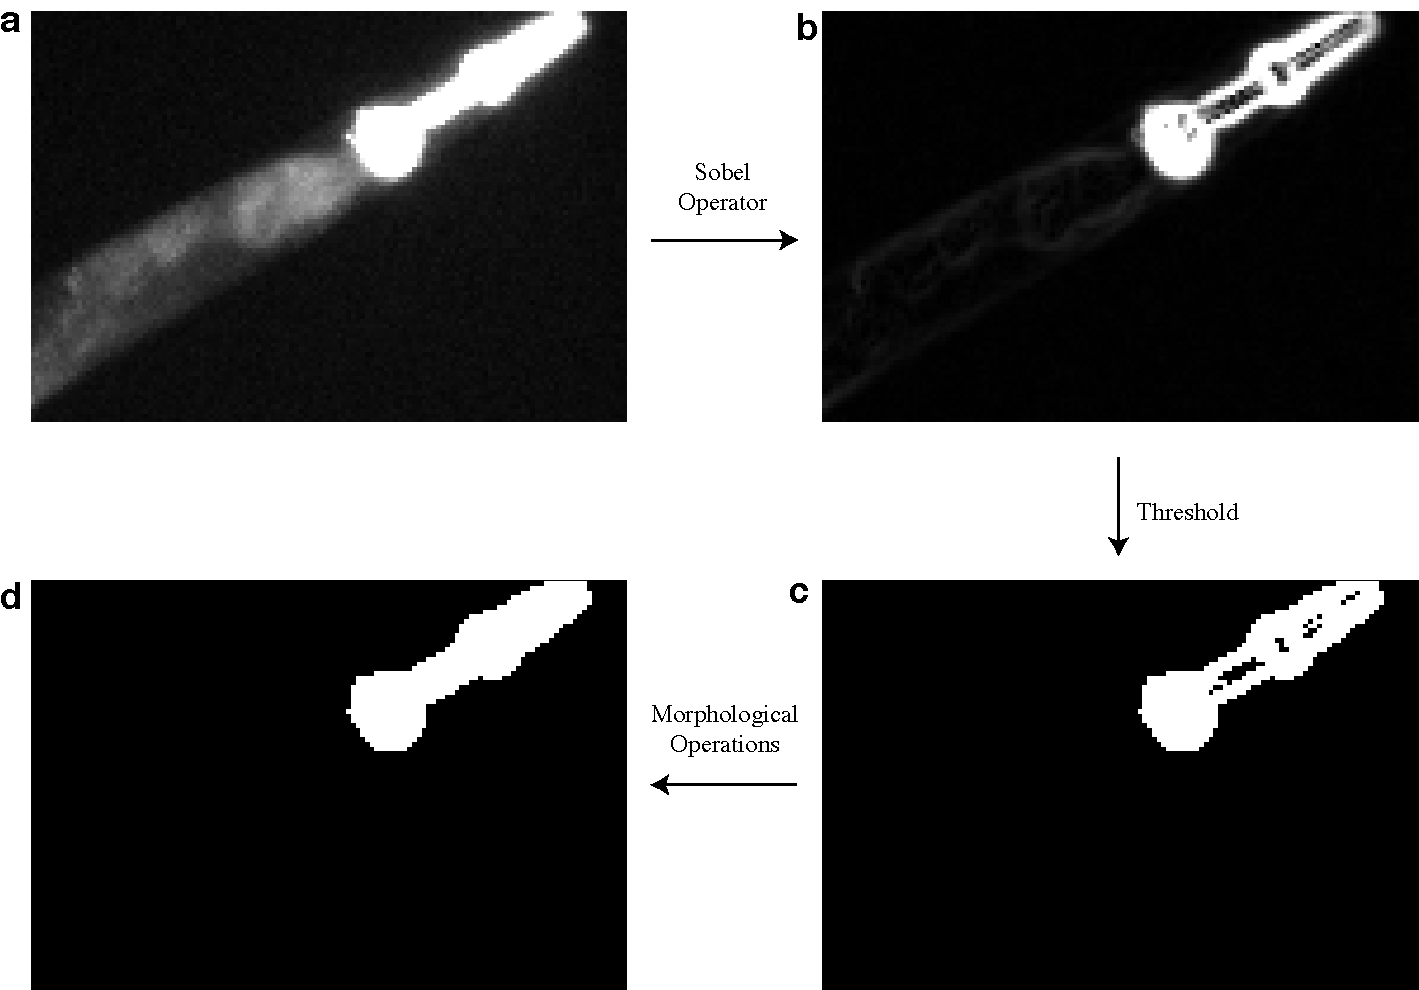
\includegraphics[scale=.40]{Figures/rendered_files/sobel}
    \decoRule
    \caption[Overview of the improved segmentation algorithm]{An overview of the improved segmentation algorithm. \textbf{a} The original image, displaying fluorescence of roGFP in the pharynx and the autofluorescence of the gut. \textbf{b} The resultant image after application of the sobel operator. \textbf{c} The resultant binary image after thresholding the edge-emphasized image. \textbf{d} The final segmented binary image, after performing morphological cleaning operations.}
    \label{fig:NewPipeline}
\end{figure}

For reasons described in \ref{TLMidlines}, an image taken with transmitted light must also be segmented. Even though the distribution of intensities in transmitted light images are very different from fluorescence images, this edge-based segmentation algorithm still performs robustly (Figure \ref{fig:TLSeg}). This highlights another benefit of the improved method: image brightness independence. If one strain's pharynx fluoresces dimly, an edge-based segmentation method still performs well while the static thresholding method requires the manual change of the threshold parameter.

\begin{figure}[ht]
    \centering
    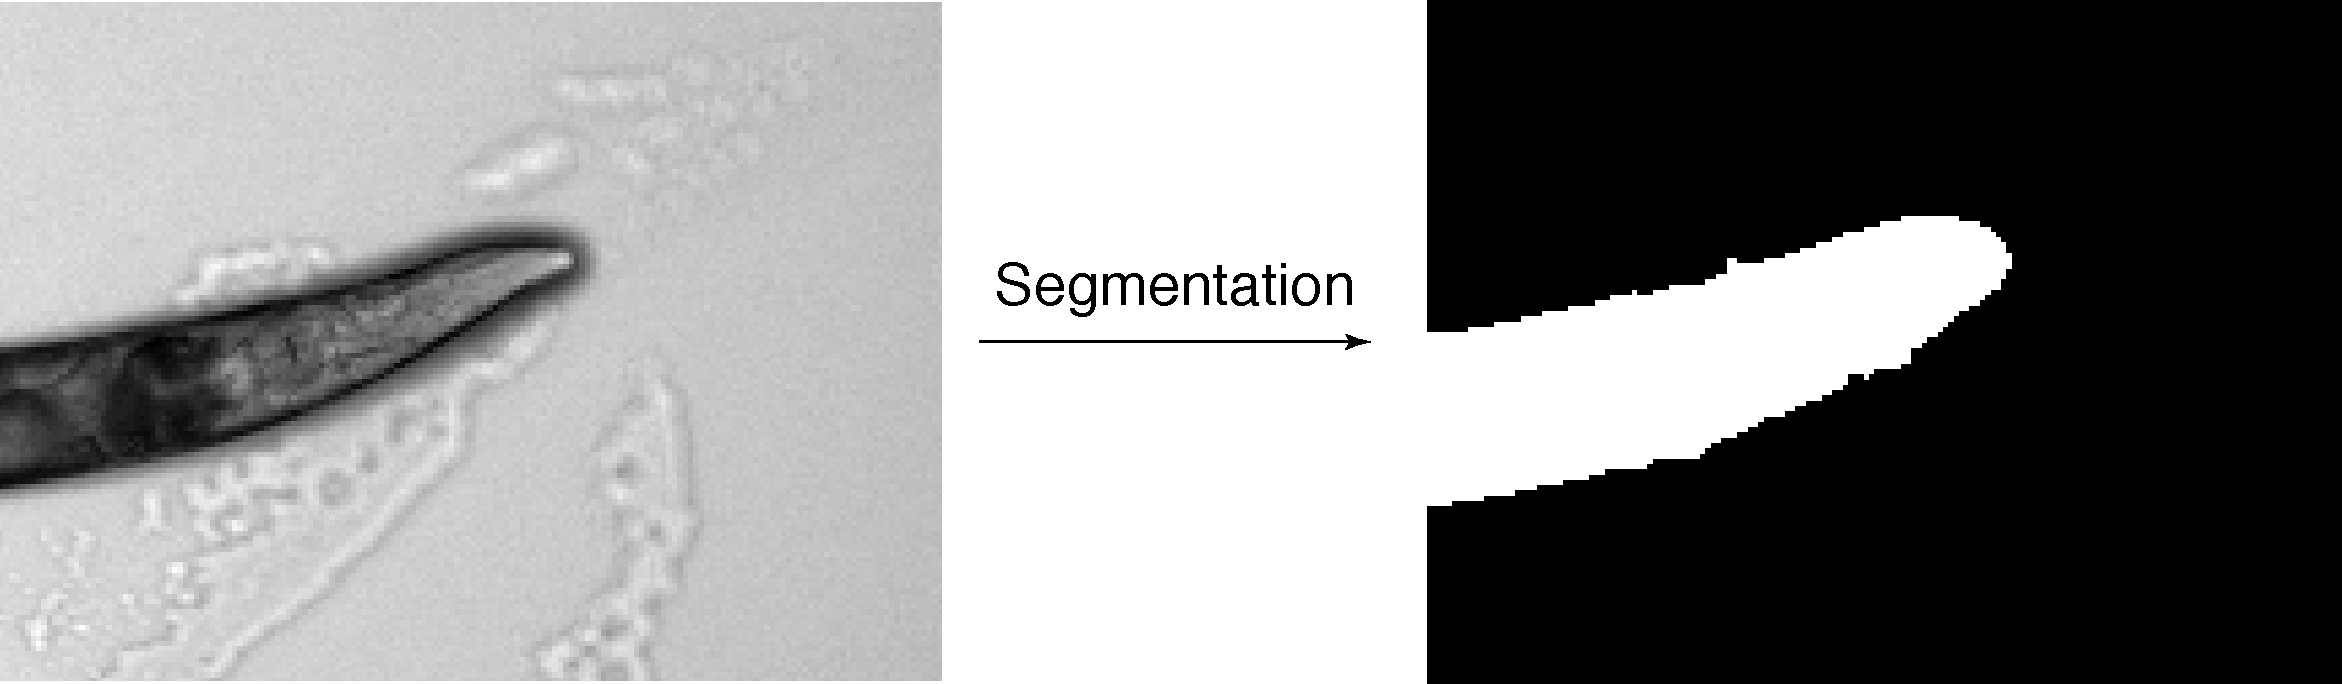
\includegraphics[scale=.30]{Figures/rendered_files/tl_segmentation}
    \decoRule
    \caption[Segmentation of a transmitted-light image]{Segmentation of a transmitted-light image}
    \label{fig:TLSeg}
\end{figure}

%-------------------------------------------------------------------------------------
%	SECTION 2
%-------------------------------------------------------------------------------------
\section{Flexible measurement boundaries account for anterior-posterior movement} \label{channelSegmentation}

As described in \ref{limitations}, inter-frame movement is a large source of error. To understand why, consider the how the previous pipeline takes measurements. First, a single mask using the image taken at 410 nm is computed. This mask is then applied to both the 410 nm and 470 nm images. Pixels corresponding to \texttt{1} in the mask retain their value while pixels corresponding to \texttt{0} in the mask are assigned the value \texttt{0}. Measurements are taken of the masked images. Thus, if the animal pumps, measurement might start in the gut or halfway through the posterior bulb, depending on if the animal contracted during the first or second frame. If the animal contracts during the first frame and extends in the second, the mask will be too "short" and measurement in the second frame will start in the middle of the posterior bulb. If the animal is extended in the first frame and contracts in the second, the mask will be too "long" and measurement in the second frame will start in the gut. This error is accounted for via visual inspection of ratio images so as to exclude those animals who have moved from analysis.

\begin{figure}[ht]
    \centering
    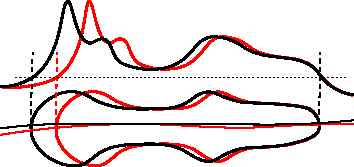
\includegraphics[scale=1.20]{Figures/rendered_files/new_boundaries_cartoon}
    \decoRule
    \caption[Flexible measurement boundaries]{A cartoon depicting the flexible measurement boundaries in the revised measurement pipeline. The first frame is depicted in black while the second is in red.}
    \label{fig:NewBoundariesCartoon}
\end{figure}

The new approach (summarized graphically in Figure \ref{fig:NewBoundariesCartoon}) tries to account for this movement without the need for manual exclusion. Here, segmentation masks are not applied to the images before measurement as before. Instead, they are used only in the calculation of the midlines (described in \ref{Midlines}). Intensity profiles of the unmasked images are taken under the midlines. The intensity profiles are trimmed to the point where they cross a threshold then resized to the same length via linear interpolation. Allowing measurement boundaries to move flexibly is a simple yet effective change in reducing error introduced by inter-frame pharyngeal contractions.

%-------------------------------------------------------------------------------------
%	SECTION 3
%-------------------------------------------------------------------------------------
\section{Midlines} \label{Midlines}

The previous centerline estimation algorithm takes as input an image of the segmented pharynx aligned horizontally along its anterior posterior axis and works as follows (depicted in figure \ref{fig:oldMidline}).

\begin{figure}[ht]
    \centering
    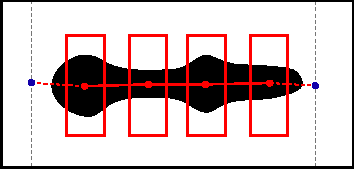
\includegraphics[scale=1.5]{Figures/rendered_files/old_midline_algorithm}
    \decoRule
    \caption[Previous centerline estimation algorithm]{Cartoon representation of the previous centerline estimation algorithm.}
    \label{fig:oldMidline}
\end{figure}

Boxes are drawn at specific static coordinates. The centroid of each shape is calculated (red points). Lines (solid) connect these points. The y-coordinates of the terminating points (blue) are determined via the point-slope method $y=mx+b$ where $m$ is the inverse of the slope of the neighboring line, $x$ is a fixed constant and $b$ is the y-coordinate of the neighboring point.

% SUBSECTION 
\subsection{A transmitted light image helps to anchor the midlines} \label{TLMidlines}
A major problem faced by the current centerline estimation algorithm is instability around the posterior bulb. Small positional changes in the neighboring points cause the terminal point to move dramatically. These instabilities must be manually corrected.

To address this concern, the new centerline estimation algorithm differs from the old in two ways. First, the new midline is estimated by treating the binary mask as points in coordinate space and  fitting them with a B-spline.  Second, the new midline incorporates positional information from a transmitted-light image. The algorithm is depicted graphically in Figure \ref{fig:midlineFit}. We segment both the transmitted-light and fluorescence images with the algorithm described in \ref{segMethod}, resulting in two binary masks. These masks are combined by cutting off the transmitted-light mask when the fluorescence mask starts. The combined mask is fed into the B-spline fit. The points from the transmitted-light mask serve to constrain and anchor the previously unstable posterior-bulb region of the estimated centerline. An additional benefit is that the estimated centerline is defined functionally, and is subject to functional analysis.

\begin{figure}[ht]
    \centering
    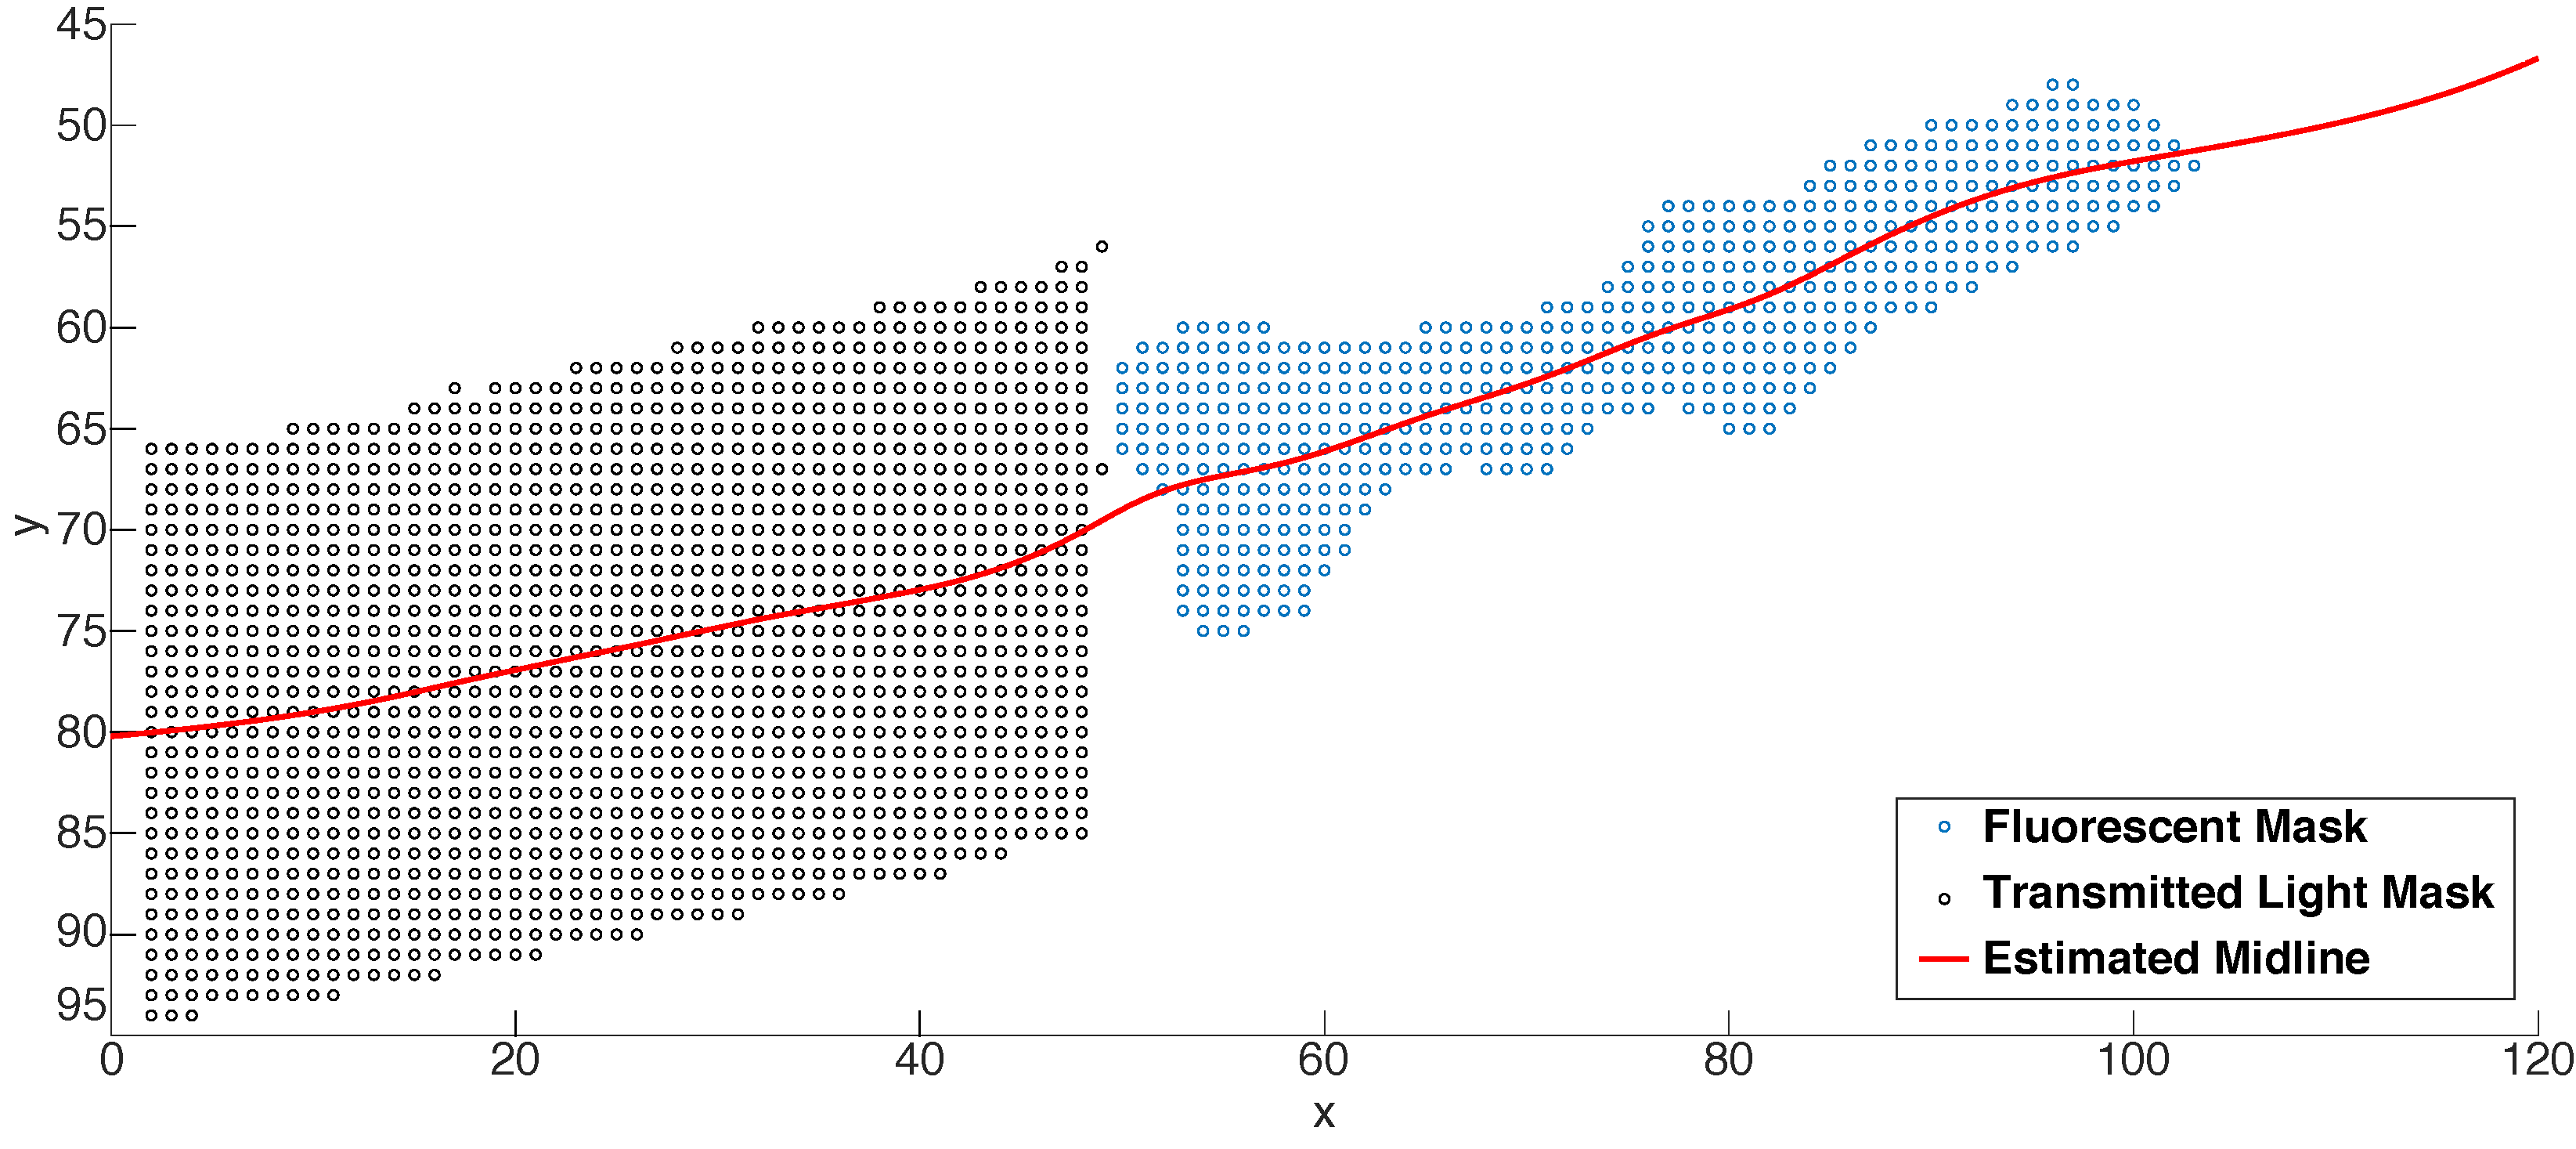
\includegraphics[scale=.25]{Figures/rendered_files/midline_fit}
    \decoRule
    \caption[Improved centerline estimation algorithm]{Depiction of the improved centerline estimation algorithm. Black points correspond to the segmented transmitted-light image, blue points correspond to the segmented fluorescence image. The estimated midline is shown in red.}
    \label{fig:midlineFit}
\end{figure}

% SUBSECTION 
\subsection{Dorsoventral tip movement is addressed with frame-specific midlines} \label{frameSpecificMidlines}
We saw in \ref{channelSegmentation} a strategy to combat the major mode of inter-frame movement, contractions of the posterior bulb. However, there is another less common mode: dorsal-ventral movement of the tip. The spline algorithm described above allows the centerline to follow the curve of the tip without human intervention. To address inter-frame movement, the new pipeline draws a midline independently in each frame.

\begin{figure}[ht]
    \centering
    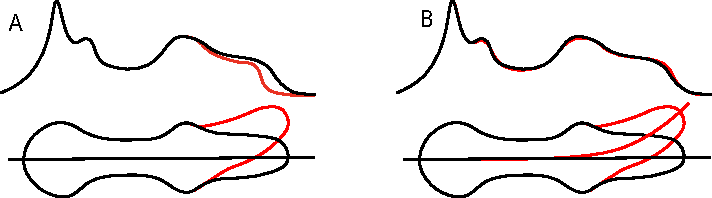
\includegraphics{Figures/rendered_files/dual_midlines}
    \decoRule
    \caption[Frame-specific midlines]{The result of using frame-specific midlines. \textbf{A} Using a single midline ignores the pharynx's curve in the second frame (red), resulting in error in the intensity profile. \textbf{B} Frame-specific midlines follow the curve of each shape, resulting in more accurate intensity profiles.}
    \label{fig:DualMidlines}
\end{figure}

%-------------------------------------------------------------------------------------
%	SECTION 4
%-------------------------------------------------------------------------------------
\section{Channel Registration picks up the slack} \label{method:Registration}

The frame-specific midline approach discussed in \ref{frameSpecificMidlines} introduces problems of its own. Specifically, the length of the intensity profile may be dilated nonlinearly due to differences in the arc length of each midline. That is, some sections of the intensity profile measured under these lines might be stretched while others are compressed. To address these nonlinear dilations, we utilized functional registration.

The goal of functional registration is to, given several curves with similar shapes, \textit{register} the curves such that salient features are aligned, but amplitude information from the original curves is unchanged. The algorithms generate a "warping function" $x_{new} = h(x)$ which maps $x$ positions along each curve to each other. Figure \ref{fig:FunctionalRegistrationCartoon} depicts this process. 

\begin{figure}[ht]
    \centering
    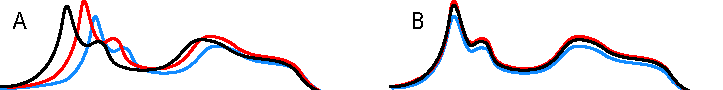
\includegraphics{Figures/rendered_files/functional_registration}
    \decoRule
    \caption[Functional registration of intensity profiles]{A visual representation of the goal of registration. The curves in \textbf{A} a are unregistered, and contain minimal amplitude variation but significant phase variation. After registration (\textbf{B}), the curves retain amplitude variation but phase variation has been removed.}
    \label{fig:FunctionalRegistrationCartoon}
\end{figure}

Our pipeline uses the MATLAB packaged fdaM \todo{link here or citation} to perform functional registration. Discrete observations are \textit{functionalized} before registration takes place. Observations were functionalized by fitting a B-spline to the discrete intensity profile. The number of knots for the spline was chosen manually, and a roughness penalty was computed using the generalized cross-validation method. One of the desirable properties of B-spline fitting is that it smooths out noise. However, we aimed to understand how registration contributes to error reduction independently of spline smoothing. 

To disentangle the effects of these operations, we register highly smoothed data to obtain a warp function, then apply that warp function to a "rough" fit of the data (Figure \ref{fig:SmoothRough}). The error is computed between the resultant warped "rough" functions.

\begin{figure}[ht]
    \centering
    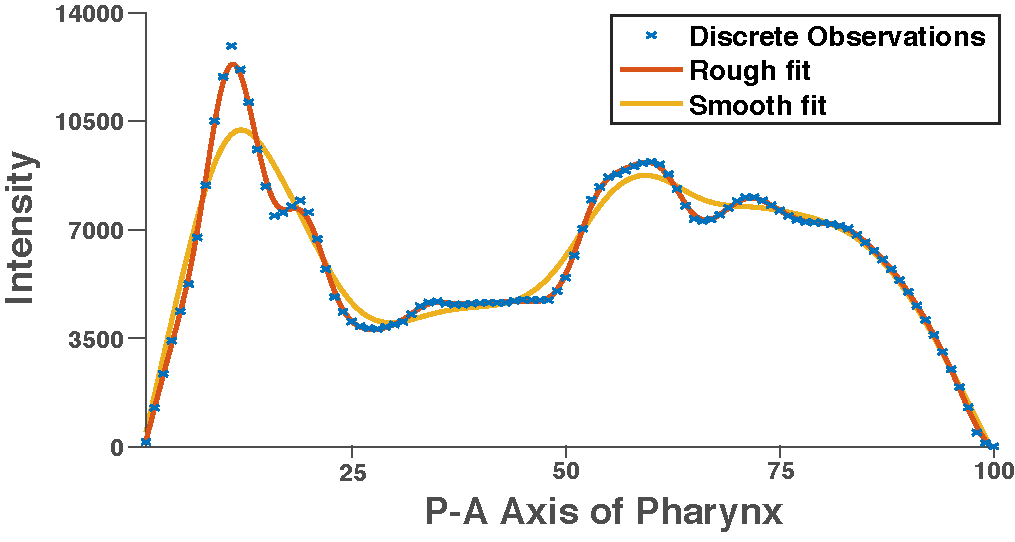
\includegraphics[scale=0.6]{Figures/rendered_files/smoothRough}
    \decoRule
    \caption[Smooth vs. rough functionalization]{Discrete observations (blue) are fit with different roughness penalties: $\lambda=6.3$ (red), $\lambda=100$ (yellow).}
    \label{fig:SmoothRough}
\end{figure}